%% 美赛模板:正文部分

\documentclass[12pt]{article}  % 官方要求字号不小于 12 号,此处选择 12 号字体

% 本模板不需要填写年份,以当前电脑时间自动生成
% 请在以下的方括号中填写队伍控制号
\usepackage[XJ210]{easymcm}  % 载入 EasyMCM 模板文件
\problem{A}  % 请在此处填写题号
%\usepackage{mathptmx}  % 这是 Times 字体,中规中矩 
\usepackage{mathpazo}  % 这是 COMAP 官方杂志采用的更好看的 Palatino 字体,可替代以上的 mathptmx 宏包
\usepackage{multicol}
\usepackage[noend]{algpseudocode}
% \usepackage[ruled]{algpseudocode}
\usepackage{algorithmicx,algorithm}
\usepackage{minted}
\title{Dynamic evolution model of finless porpoise population}  % 标题
%\usepackage{newtxtext}
%\usepackage{palatino}
% 如需要修改题头(默认为 MCM/ICM),请使用以下命令(此处修改为 MCM)
%\renewcommand{\contest}{MCM}
% 文档开始
\begin{document}
% 此处填写摘要内容
\begin{abstract}
With the intensification of modern human industrial activities, the ecological environment of the Yangtze River Basin has deteriorated sharply. 
 Based on the living habits of dolphins, human factors and natural factors such as \textbf{inbreeding recession}, disasters, and environmental capacity are taken as the constraints of population growth. Seven parameters representing \textbf{population viability} were selected, including age structure, sex ratio, population density, reproduction rate, inbreeding coefficient and survival rate of each age group.

For Model 1, considering that the ex-situ refuges have superior natural conditions, the population of dolphins can be free from the interference of human factors. Considering that the reproduction mode of porpoise is \textbf{density-constrained} and there is a trend of inbreeding depression, the \textbf{difference equations} representing population viability are constructed.

Due to the small number of Yangtze River porpoises, all life activities can be regarded as \textbf{random processes}. Due to this feature, the \textbf{hidden Markov} population evolution prediction model is constructed, and the state observation sequence from the initial population to the future population is randomly generated. The maximum probability observation sequence is obtained based on the \textbf{Viterbi algorithm}, and it is substituted into the established state transition equation. The number of dolphin population in the reserve 20 years in the future is \textbf{271}, and the initial population growth rate is about \textbf{9.3 \%}, the average population growth rate is \textbf{6.8 \%}.

By adjusting the sex ratio of the initial state, it is found that when the sex ratio is less than 0.5, the population number decreases first and then increases, showing an \textbf{V type}, and the lower the sex ratio is, the later the lowest population number occurs ; when the proportion of males and females was greater than 0.5, it showed \textbf{a single ladder}. The growth rate of the number of porpoises slightly decrease with the increase of years, and finally stabilized at a high level. The reason for this phenomenon is that the population growth rate is mainly attributed to the proportion of female individuals, and the sex ratio of newborn dolphins is close to 1 : 1, so the population change curve tends to the growth curve of the sex ratio of 1 : 1.

For Model 2 , in the non-protected area, the environmental capacity is a function of decreasing over time, and the impact of human factors and natural disasters also need to be considered. Due to the short lifespan of dolphins, human factors can be considered as a constant. Similarly, the difference equations of the survival ability of the Yangtze porpoise population in the non-protected area can be constructed. Then, the HMM population prediction model is used to solve the problem. It is found that Yangtze finless porpoise will functionally extinct in \textbf{2035} if proper protection measure is not taken.

Finally, based on the results of those two demographic models stated above, some constructive suggestions on the protection of Yangtze porpoise were put forward at the end of the paper.

\noindent%取消单段缩进
\textbf{Keywords: }finless porpoise; population viability; Hidden Markov; sex ratio
\end{abstract}
\maketitle  % 生成 Summary Sheet
\tableofcontents  % 生成目录



%\usepackage{mathpazo}  % 这是 COMAP 官方杂志采用的更好看的 Palatino 字体,可替代以上的 mathptmx 宏包
% 正文开始
\section{Introduction}%1 introduction
\subsection{Problem background}%1.1 Problem background

  Following the extinction of the Baiji, the finless porpoise has become the only freshwater mammal in the Yangtze River. Currently, it is mainly distributed in the middle and lower reaches of the Yangtze River and the waters of Dongting Lake and Poyang Lake. However, due to the deterioration of the living environment, the population of Yangtze River dolphins has dropped sharply in the past 20 years and the dolphins are on the verge of extinction. The number of Yangtze finless porpoises dropped from more than 2,700 to 1,012 from 1991 to 2018. 

Since the 1980s, Chinese government has successively established five ex-situ refuges and has adopted three major protection measures: in-situ protection, ex-situ protection and artificial breeding. Because of that, the latest report shows that the population of the Yangtze finless porpoise has steadily increased, but its endangered situation has not changed.
\begin{figure}[htbp]%插入图片
	\small
	\centering
	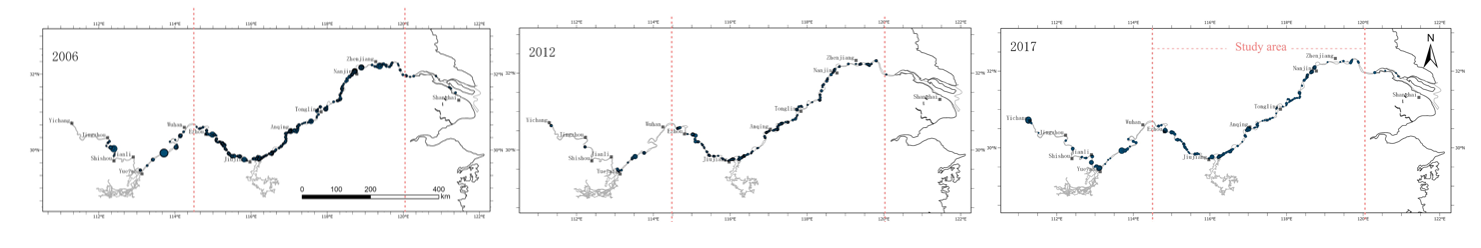
\includegraphics[height=4cm,width=16cm]{figures/num_changes.png}%图片名
	\caption{Population distribution of finless porpoise in 2006, 2012 and 2017}%\label{fig:7}%题注
\end{figure}
\subsection{Restatement of the Problem}%1.2Overview of our goals

%Since the 1980s, my country has successively established five ex situ protected areas by adopting three major protection measures: in situ protection, ex situ protection and artificial breeding. The latest report shows that the population of the Yangtze finless porpoise has steadily increased, but its critically endangered status has not changed.
\begin{itemize}%前面圆点。开头
	\item Establish a mathematical model to predict the population of the Yangtze finless porpoise after 20 years in those five ex-situ refuges. The model needs to show how much the sex ratio of the 150 finless porpoises in the ex-situ refuges will affect the development of the finless porpoise population.
	\item On the basis of the first question, discuss whether the Yangtze finless porpoise will become functionally extinct if ex-situ conservation measures are not taken. If the Yangtze finless porpoise will become functionally extinct in the future, try to predict the exact time of its functional extinction.
	\item Based on the previous analysis and results, give some constructive proposals for the protection of Yangtze finless porpoise of no more than two pages and submit it to the relevant departments.
\end{itemize}

\section{General Assumptions and Model Overview}%2 Assumptions
%\noindent%取消单段缩进
%\textbf{General Assumptions}

To simplify the problem, we make the following basic assumptions, each of which is properly justified.

\begin{itemize}
	\item \textbf{ Assumptions 1:}Fertility of mature female finless porpoise independent of age.
	
$\hookrightarrow$ \textbf{Justification:}The reproductive capacity of female finless porpoises after sexual maturity varies among different age groups, but the average reproductive capacity of mature females of the entire population is basically the same every year.
	\item \textbf{ Assumptions 2:}Ex-situ refuges are free from external adverse factors.
	
$\hookrightarrow$ \textbf{Justification:}In ex situ protected areas, there are basically no adverse factors such as fishing, shipping, pesticide pollution and major natural disasters.

\end{itemize}

\section{Glossary and Notation}  % 3 Data Processing
\subsection{Glossary}
\begin{itemize}%前面圆点。开头
	\item \textbf{Genetic drift: }refers to the cumulative and non-adaptive fluctuation in allele frequencies resulting from the random sampling of genes in each generation. 
	\item  \textbf{Functional extinction: }means the situation in which a certain type of organism living under natural conditions, its population is reduced to such a state that cannot sustain its reproduction;

\end{itemize}
\subsection{Notation}
The primary notations used in this paper are listed in \textbf{Table \ref{Ntt}}. There can be some
other notations to be described in other parts of the paper.
\begin{table}[!htbp]
\begin{center}
\caption{Notations}
\begin{tabular}{cl}
    \toprule
    \multicolumn{1}{m{3cm}}{\centering Symbol}
    &\multicolumn{1}{m{8cm}}{\centering Definition}\\
    \midrule
   ${{F}_{is}}$&inbreeding coefficient\\
    ${{s}_{ij}}$&Survival rate by age\\
   $D(t)$&population density\\
    ${{\omega }_{\text{ij}}}$&The proportion of individuals in i age group\\
    $\eta $&The ratio of the number of males and females\\
    \bottomrule
\end{tabular}\label{Ntt}
\end{center}
\end{table}
%\section{Data Processing}  % 3 Data Processing

%By analyzing the data in the table, we find that some data are zero for a period of time, which we regard as missing data. In order to solve this problem, we use cubic spline method for interpolation fitting to fill in the exact data and ensure the data integrity.

\section{Model preparation}

\subsection{Overview of Finless Dolphin Habits}
Related studies have shown that the mating mode of Yangtze River porpoise is polygamy, and the average age of female and male porpoises’ sexual maturity is about 5 years old\upcite{1}. The highest reproductive age is about 16 years old, and the sex ratio at birth is 1:1 under normal conditions. The mode of the porpoise’s population growth is density-dependent, that is, the probability of mature females participating in reproduction varies with the proportion of females and population density.

\subsection{Population growth constraints}
\subsubsection{Human Factors }
\textbf{\S \ Environmental capacity $K(t)$: }For finless porpoises living in the wild, due to the influence of human activities, the environmental carrying capacity of the waters in which they live decreases $2\%\sim 3\%$ year by year.

\textbf{\S \ Shipping business: }Studies have shown that young porpoises are sensitive to the interference of underwater noise caused by the ships’ engine. To be more specific, because the young porpoise does not have the sonar ability, noise interference may lead to the loss of contact between the young porpoise and its parent porpoise, thereby reducing its survival ability and even directly leading to its death.

\textbf{\S \ Fishery: }Fishery will lead to the decrease of dolphins’ food, and fishing tools will also have a devastating blow to dolphins. Excessive fishing also aggravates the difficulty of dolphin survival. According to the records, 20 deaths were recorded in 2008, 21 deaths were recorded in 2009, 27 deaths were recorded in 2010, 21 deaths were recorded in 2011, 21 deaths were recorded in 2012.

\textbf{\S \ Water pollution: } Studies have shown that water pollution will reduce the reproductive capacity of Yangtze River porpoise. Some chemical raw materials or wastewater will affect the breeding ability of dolphins, resulting in low birth rate. Also, researchers point out that water pollution will also lead to unbalanced sex ratio of newborns. This will also give rise to the decrease of population in the long term.
\begin{figure}[htbp]%插入图片
	\small
	\centering
	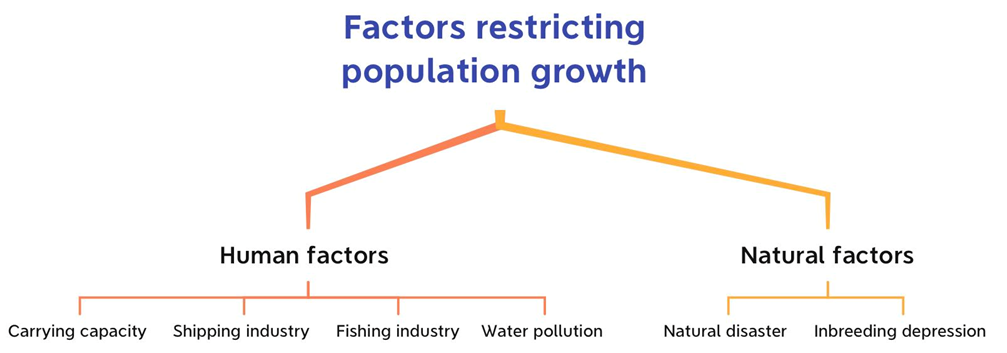
\includegraphics[height=4cm,width=10cm]{figures/Cons2.png}%图片名
	\caption{Constraining factors of finless porpoise population growth}%\label{fig:7}%题注
\end{figure}

\subsubsection{Natural Factors }
\textbf{\S \ Inbreeding depression: }Many studies of laboratory, domestic, and zoo animals have documented reduced survival and fecundity of in- bred young. Inbreeding depression\upcite{2} is thus a major concern in the management of small populations.
Ex-situ reintroduction refuges can increase local porpoise population numbers, but long-term maintenance of small, isolated porpoise populations in such refuges may lead to loss of genetic diversity and increased risk of inbreeding depression.

\textbf{\S \ Natural disaster: }In addition to human factors, the snow disaster in 2008, the extremely low water level of the Poyang Lake drought in 2019, as well as accidents and other disasters still exist.  

\subsection{Determination of population parameters}
\textbf{\S \ age structure ${{\omega }_{\text{i}}}(t)$: }Although some finless porpoises can stay alive for more than 16 years, they are just a very small part of the whole community. So we think that the age of finless porpoise ranges from 0 to 16. The number of porpoises who are in the age of i is  ${{\omega }_{\text{i}}}(t)$.

\textbf{\S \ Female ratio $\eta (t)$: }In the community of porpoise, female porpoises take up $\eta (t)$ of the whole community. Relatively, the male porpoises take up 1-$\eta (t)$.It is worth emphasizing that the probability of adult female finless porpoise participating in reproduction is affected by the proportion of both males and females in the population.

\textbf{\S \ Population density $D(t)$: }For a specific water area,  as the population increases, the degree of mutual influence between individuals begins to increase, its quantitative expression is $D(t)=N(t)/K(t)$.

\textbf{\S \ Reproductive rate $b(t)$: }Combined with official data, the maturity time is $\Delta {{t}_{mature}}=5$, the reproductive years after maturity is $\Delta {{t}_{breed}}=11$, and the production interval of mature females is $\Delta {{t}_{birth}}=1.42$, so the maximum reproductive rate of the population is:
\begin{equation}%\label{eq:heat}
{{b}_{\max }}=\frac{{{\eta }_{f}}\Delta {{t}_{breed}}}{(\Delta {{t}_{mature}}+\Delta {{t}_{\text{br}eed}})\Delta {{t}_{birth}}}
\end{equation}
\textbf{\S \ Reproductive rate $b(t)$: }
The population growth of the finless porpoise is density-constrained\upcite{3}, so the reproductive probability of mature females is not only affected gender ratio in the population, but also proportional to the population density in the active waters. Therefore $b\propto D,{{\eta }_{f}},{{\eta }_{m}}$, the expression of the population reproductive rate is obtained:
\begin{equation}%\label{eq:heat}
b(t)={{f}_{1}}(N/K)\cdot {{f}_{2}}({{\eta }_{m}})\cdot \frac{{{\eta }_{f}}\Delta {{t}_{breed}}}{(\Delta {{t}_{mature}}+\Delta {{t}_{\text{br}eed}})\Delta {{t}_{birth}}}
\end{equation}

\textbf{\S \ Inbreeding coefficient ${{F}_{is}}(t)$: }Finless porpoises are social animals, so the probability of inbreeding is proportional to the population density in the area ${{F}_{is}}\propto D$.

\textbf{\S \ Survival rate by age ${{s}_{ij}}(t)$: }According to the logarithmic model developed by Morton et al. (1956), the survival rate of juvenile finless porpoise satisfies the following formula:
\begin{equation}%\label{eq:heat}
\ln S=-A-B{{F}_{\text{is}}}
\end{equation}
$A$ :The logarithm of survival without inbreeding;$B$ :A measure of the rate at which survival decreases with inbreeding.Rall et al. studied the lethal equivalence coefficient of 40 mammalian populations and found that each diploid had 3.14 lethal equivalents, so $B=3.14$.

\section{Model 1 : HMM prediction model of finless porpoises in protected areas}
\subsection{Analysis of characteristics in protected areas}
\textbf{Not affected by human factors: }
The ex-situ refuges have favorable natural environment, so that dolphins can be protected from human factors such as fishing industry, shipping business and water pollution.

\textbf{Inbreeding depression has an impact: }
With the continuous development of population, inbreeding depression is becoming more and more obvious. Therefore, the influence of inbreeding on the survival rate of the offspring needs to be carefully considered.
\begin{figure}[htbp]%插入图片
	\small
	\centering
	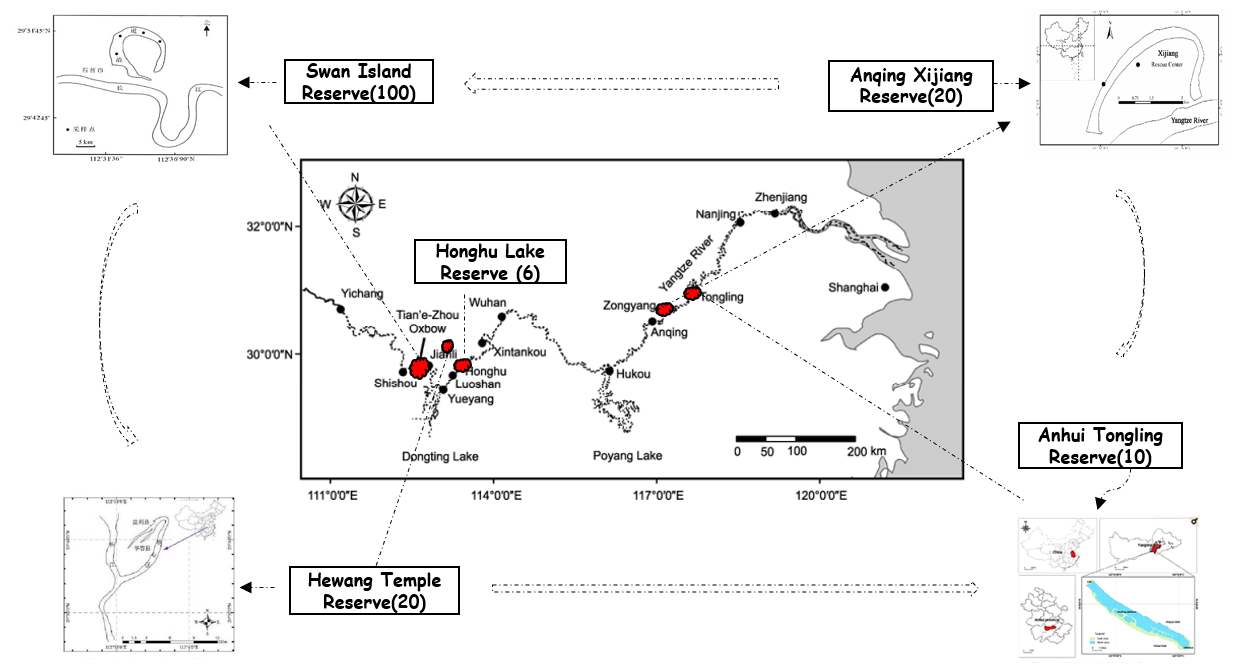
\includegraphics[height=6cm,width=10cm]{figures/5prot.png}%图片名
	\caption{Distribution map of five ex situ protected areas}%\label{fig:7}%题注
\end{figure}

\textbf{The environmental capacity is basically constant, ignoring environmental resistance: }
We believe that, for the whole of the five major ex-situ refuges, the environmental capacity is large enough. Therefore, we ignore the environmental resistance brought by environmental capacity.


\subsection{Construction of Difference Equation of Population Viability}
\noindent%取消单段缩进
\bullet
\textbf{ Initial population value}

Combined with the survey data, we can obtain the initial value of the population $N(0)$,the proportion of each age group $W(0)=\left[ {{\omega }_{1j}}(0),{{\omega }_{1j}}(0),\cdots ,{{\omega }_{16j}}(0) \right]$.

\noindent%取消单段缩进
\Rightarrow 
\textbf{Population mortality}

Combined with the survival rate, the mortality rate of individuals of different ages can be obtained as $(1-{{s}_{ij}})$.The total number of deaths in the group $\Delta {{N}_{death}}$ is equal to the sum of the number of deaths in each age group.Therefore, the number of dead individuals of the finless porpoise population from the $t$ to the $t+1$ year is:
\begin{equation}%\label{eq:heat}
\Delta {{N}_{death}}(t,t+1)=\sum\limits_{i=0}^{16}{N(t){{\omega }_{i-1j}}(t)(1-{{e}^{-A-B{{F}_{is}}(t)}})}
\end{equation}
\begin{figure}[htbp]%插入图片
	\small
	\centering
	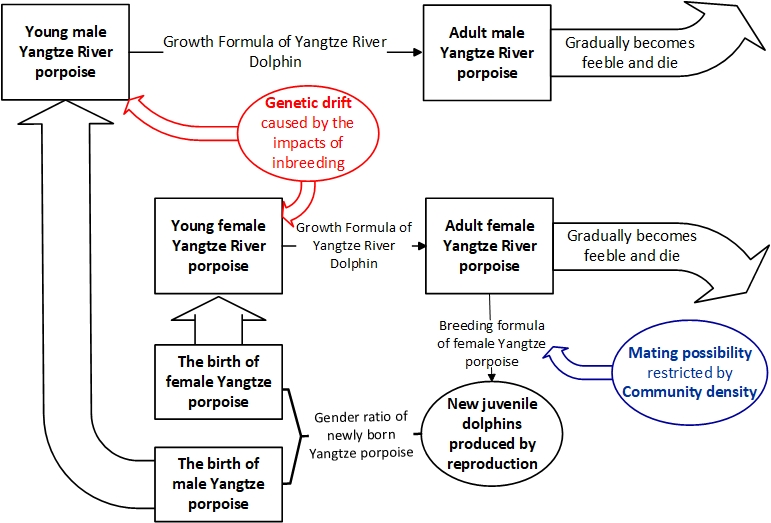
\includegraphics[height=7cm,width=10cm]{figures/VortexM1.jpg}%图片名
	\caption{Dynamic evolution process of protected area population}%\label{fig:7}%题注
\end{figure}
\noindent%取消单段缩进
\Rightarrow  
\textbf{Number of newborn dolphins}

Since the number of newborn finless porpoises in the finless porpoise population $\Delta {{N}_{birth}}$ from $t$ to $t+1$ will be equal to the number of female finless porpoises $N{{\omega }_{i0}}$ in the age range of 5-16 multiplied by the years of a single mature female reproductive rate $b(t)$.
Combined with formula (2), the expression of population annual growth can be obtained :
\begin{equation}%\label{eq:heat}
\Delta {{N}_{birth}}(t,t+1)=\sum\limits_{i=5}^{16}{N(t){{\omega }_{i1}}(t)\frac{{{f}_{1}}(N/K)\cdot {{f}_{2}}({{\eta }_{m}})\cdot {{\eta }_{f}}\Delta {{t}_{breed}}}{(\Delta {{t}_{mature}}+\Delta {{t}_{\text{br}eed}})\Delta {{t}_{birth}}}}
\end{equation}

\noindent%取消单段缩进
\Rightarrow 
\textbf{Population number sequence}

Therefore, the total number of finless porpoises in the reserve in year t+1 is $N(t+1)=N(t)+\Delta {{N}_{birth}}(t,t+1)-\Delta {{N}_{death}}(t,t+1)$.The number of deaths and the number of new individuals obtained above are used to obtain the final expression of the number of the population in the year:
\begin{equation}%\label{eq:heat}
N(t+1)=N(t)-\sum\limits_{i=1}^{16}{N(t){{\omega }_{i-1j}}(t)(1-{{e}^{-A-B{{F}_{is}}(t)}})}+\sum\limits_{i=5}^{16}{N(t){{\omega }_{i0}}(t)\cdot b(t)}
\end{equation}

\noindent%取消单段缩进
\Rightarrow 
\textbf{Intermediate iterative relationship}

The iterative relationship of age structure needs to be discussed in two cases.The individual condition of the $0\sim 1$ age group is completely determined by the newborn puppies of the previous year,and the sex ratio is 1:1.
The proportion of age group $i\sim i+1(2\le i\le 16)$ in the population is equal to the proportion of age group $i-1\sim i$ in the previous year multiplied by its survival rate ${{s}_{i-1j}}$ , so the age structure of year $t+1$ is obtained as follows:
\begin{equation}
\begin{align*}
\begin{split}
{{\omega }_{ij}}(t+1)= \left \{
\begin{array}{ll}
{\Delta {{N}_{birth}}(t,t+1)}/{N(t+1)},   & i=1\\
{{\omega }_{i-1j}}(t)\cdot (1-{{e}^{-A-B{{F}_{is}}}}),     & i=2,3,\cdots ,16
\end{array}
\right.
\end{split}
\end{align*}
\end{equation}

\subsection{Hidden Markov Population Prediction Model}
\subsubsection{Background of HMM Predictive Models}
With the exception of aging, virtually all events in the life of an organism are stochastic. Mating, reproduction, gene transmission between generations, migration, disease and predation can be described by probability distributions. Small samples like finless porpoise display high variance around the mean, so the fates of small wildlife populations are often determined more by random chance than by the mean birth and death rates that reflect adaptations to their environment.

Hidden Markov Model is a probability model about time series, which describes the process of randomly generating an unobservable random sequence\upcite{4} of states from a hidden Markov chain, which fully simulates the finless porpoise population. The random process of evolution describes the future survival behavior of an individual with a probability distribution.

\subsubsection{The establishment of HMM model}
In this part, we propose the Hidden Markov Model (HMM) to predict the evolution of Yangtze finless porpoise. Models discussed above are all probabilistic Model, which we cannot give a certain result by simulations. However, HMM uses theoretical analysis to give the solution of most possible sequence, and makes it possible to do further prediction.

\begin{figure}[htbp]%插入图片
	\small
	\centering
	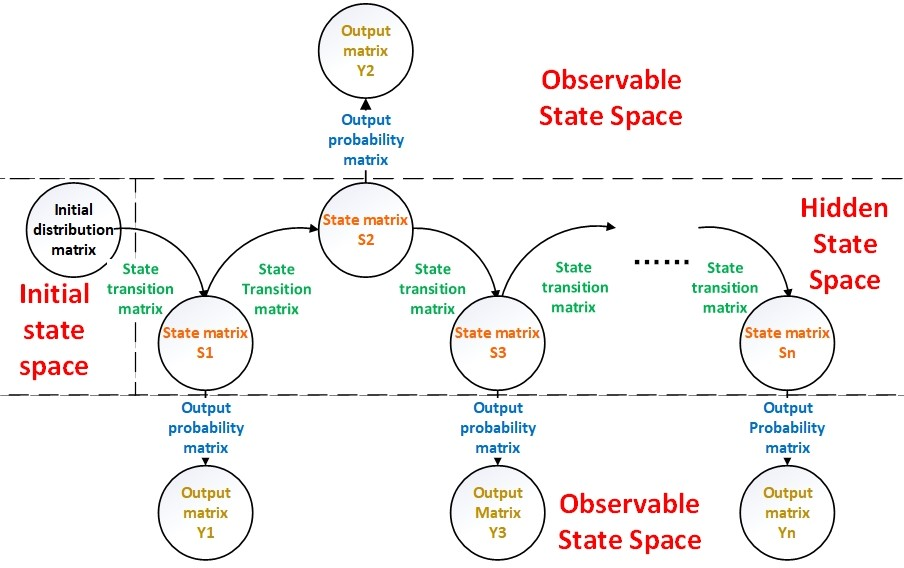
\includegraphics[height=7cm,width=11cm]{figures/HMM1.jpg}%图片名
	\caption{Schematic diagram of the HMM  prediction model}%\label{fig:7}%题注
\end{figure}

\begin{Definition}[Initial Distribution]
To represent the state of Markov Model, we introduce the State Matrix and Initial Distribution. State Matrix is what's shown below as S, while Initial Distribution is $\pi$.
\begin{equation}
S = 
\left[
\begin{matrix}
    1 & s_{0,1} & s_{0,2} & ... & s_{0,16} \\
    1 & s_{1,1} & s_{1,2} & ... & s_{1,16}
\end{matrix} \right
]. \\
\end{equation}
\begin{equation}
S_0 = \{ s_{g,a} \}|_{t=0} = \pi =
\left[
\begin{matrix}
    1 & \pi_{0,1} & \pi_{0,2} & ... & \pi_{0,16} \\
    1 & \pi_{1,1} & \pi_{1,2} & ... & \pi_{1,16}
\end{matrix} \right] . 
\end{equation}
For $s_{g,a}$ in S, g $\in gender\{ male(0),female(1) \}$ , a $\in$ age([1,16]), and $s_{g,a}$ means State Matrix in gender g , age a .For further discussion, we divide S into $S^0$ and $S^1$ by rows.
In the second formula, $\pi_{g,a}$ = N $\cdot$ P(g,a). N means total number of Yangtze River porpoise, and P(g,a) means the distribution in gender and age.
\end{Definition}

\begin{Definition}[State Transition Matrix]
The State Matrix is closely relative with time, so it's necessary to describe how it changes by time. State Transition Matrix tells the relationship between a current state and a next time state, which is shown below as $P_t$.
\begin{equation}
P_t = 
\left[
\begin{matrix}
    P(S_{t-1,0}) & 0 & ... & 0 \\
    0 & P(S_{t-1,1}) & ... & 0 \\
    ... & ... & ... & ...\\
    0 & 0 & ... & P(S_{t-1,16})
\end{matrix} \right
] , 
\end{equation}
in which $S_{t,a}$ means number of Yangtze River porpoise in time t and age a. $P(S_{t,a})$ is a function which we call it State Transition Function. Especially, $P(S_{t-1,0})$ represents the Birth  Function, and $P(S_{t-1,16}) = 0$  represents the Death Function.
\end{Definition}

\begin{Definition}[Output Matrix]
To quantify the factors which impact the number of finless porpoise most, we propose the Output Matrix Y.
\begin{equation}
Y =
\left[
\begin{matrix}
    Y_1 & Y_2 & Y_3
\end{matrix} \right    
] ,    
\end{equation}
in which $Y_{1,2,3}$ represent the impacts of underwater noise, water pollution and artificial factors(such as the fishing industry)
\end{Definition}

\begin{Definition}[Output Probability Matrix]
The output at a current time is only relative with state at that time, which we can use a matrix to describe the relationship between them. The Output Probability Matrix is a time-based matrix marked with $Q_t$.
\begin{equation}
Q_t = 
\left[
\begin{matrix}
    Q_1(S_{t,0}) & Q_2(S_{t,0}) & Q_3(S_{t,0}) \\
    Q_1(S_{t,1}) & Q_2(S_{t,1}) & Q_3(S_{t,1}) \\
    ... & ... & ... \\
    Q_1(S_{t,16}) & Q_2(S_{t,16}) & Q_3(S_{t,16})
\end{matrix} \right
] ,
\end{equation}
in which $S_{t,a}$ means number of Yangtze River porpoise in time t and age a. $Q_{1,2,3}(S_{t,a})$ are functions which represent changes on underwater noise, water pollution and artificial factors in the case of Yangtze River porpoise.
\end{Definition}

\begin{Definition}[Observation Equation]
Observation Equation gives the relationship between State Matrix, Output Probability Matrix and Output Matrix, which is shown below.
\begin{equation}
\begin{aligned}
Y^0_t = S^0_t Q_t, \\
Y^1_t = S^1_t Q_t. 
\end{aligned}
\end{equation}
$Y^a_{t}$ shows the Output Matrix in age a, time t. $Q_t$ is the Output Probability Matrix. Observation Equation describes how Output Matrix changes with the time.
\end{Definition}

\begin{Definition}[Most Possible Sequence]
All the definitions above are prepared for Most Possible Sequence. In this paper, our goal is to predict the number of finless porpoise, which is a sequence in the case of given conditions. We'll give the definition of Most Possible Sequence and propose Subsequence Theorem, as it makes probability easier to calculate.
\begin{equation}
{{s}^{*}}=\argmax_{s \in S}P(s|y).
\end{equation}
In the equation above, $s^*$ is the Most Possible Sequence, and y means exact value observed by observer. Notice that both s and y are sequence of matrices. This equation has a certain meaning, the Most Possible Sequence should be the state sequence which is most likely to happen when the observation sequence is given; therefore achieve the best prediction to the state sequence.
\end{Definition}

\begin{Theorem}[Subsequence Theorem]
\begin{equation}
\begin{aligned}
s^* &= \argmax_{s \in S}P(s|y) =  \max_{s_1,...,s_n}P(s_1,...,s_t,...,s_n,y_1,...,y_t,...,y_n)\\
&= \max_{s_t,s_{t+1},...,s_n}[P(s_{t+1},...,s_n,y_{t+1},...,y_n|s_t)\cdot \max_{s_1,s_2,...,s_{t-1}} P(s_1,...,s_{t-1},y_1,...,y_t)].
\end{aligned}
\end{equation}
\end{Theorem}

\subsubsection{Determination of initial value}
Combined with Zhang Xianfeng's literature and related survey results, the age structure of the Yangtze finless porpoise${{\omega }_{\text{ij}}}(0)$ and the corresponding survival rate ${{s}_ {ij}}(0)$, annual female reproductive rate $b(0)\approx 25\%$, male-to-male ratio $\eta (0)=1:1.12$, inbreeding coefficient ${{F}_{is} }(0)=0.25$,Therefore, the values of $A=0.33$ and $B=2.34$ are obtained by fitting.Initial populations of finless porpoises in five ex situ protected areas and initial data are listed in \textbf{Table \ref{Ntt}}. 

\begin{table}[!htbp]
\centering  
	\caption{Initial value of population parameter}
	
	\label{table_time}
	
	\begin{tabular}{cc|ccc}  
		
		\toprule   
		protected areas&Number &Age Range&Age Structure ${{\omega }_{\text{ij}}}(0)$  &Survival Rate ${{s}_{ij}}(0)$\\ 
		
		\midrule   
	Swan Island Reserve&85&	$0\sim 1$&16 \% &82\% \\ 
	Hewang Temple Reserve&21&$1\sim 2$&16 \% &86 \% 	\\  
	Anqing Xijiang Reserve&19&$2\sim 3$ & 5.5 \% &95\%  
		\\    
	Anhui Tongling Reserve&8&$3\sim 4$ &8.5 \% & 97\%	\\
	 Honghu Lake Reserve &6 &$>5$& 45 \% &94\%
		\\
		\bottomrule  
		
	\end{tabular}
\end{table}

\subsubsection{Viterbi algorithm to solve the model}

%\noindent%取消单段缩进

%\textbf{Viterbi algorithm}

We learned from Subsequence Theorem that the problem of Most Possible Sequence can be divided into several subproblems. This is a great insight, which hints that we can use dynamic programming (DP) to solve the sequence of HMM.

We first introduced the Viterbi algorithm. The Viterbi algorithm is a dynamic programming algorithm for obtaining the maximum a posteriori probability estimate of the most likely sequence of hidden states—called the Viterbi path—that results in a sequence of observed events. --(This part is from Wikipedia, remember to cite it and remove me)--

%Before giving the steps of Viterbi algorithm, we give a theoretically analysis of the entire process.

\begin{Definition}[Recursion Factor] 
To simplify expression, we use Recursion Factor to replace the original equation.
\begin{equation}
\gamma_t(i)=\max_{s_1,s_2,...,s_{t-1}}P(s_1,...,s_{t-1},s_{t=i},y_1,y_2,...,y_t).    
\end{equation}

\end{Definition}

\begin{Theorem}[Recursion Equation] 
\begin{equation}
\gamma_{t+1}(j) = \max_i ( P(s_{t+1}=j|s_t=i) \cdot \gamma_t(i) )P(y_{t+1}|s_{t+1}=j) , \ i,j \in S   
\end{equation}

\end{Theorem}

Thm 5.7.1 (Recursion Equation) provides with the theoretical support to dynamic programming. Based on the Recursion Equation, probability of states in time t+1 can be converted from it in in time t, which means recursion is available to calculate probability of states from beginning to the end.


\begin{algorithm}[]
\caption{Viterbi algorithm}
\hspace*{0.02in} {\bf Input:}
input parameters $\pi ,Y , P, Q$\\
\hspace*{0.02in} {\bf Output:} 
$s^*={s^*_1,s^*_2,...,s^*_n}$
\begin{algorithmic}[1]
\State
Let $\gamma_t(i)=\max_{s_1,s_2,...,s_{t-1}}P(s_1,...,s_{t-1},s_{t=i},y_1,...,y_t)$ \\
Initialization:
\For{each state $s_i$}
    \State $\gamma_1(i) \xleftarrow{} \pi_i q_{i y_1}$
    \State $T_2(1,i) \xleftarrow{} 0$
\EndFor
\State Recursion:
\For{i$\xleftarrow{}$2,3,...,T}
  \For{each state $s_j$}
        \State $T_1[j,i] \xleftarrow{} \max_k(T_1[k,i-1] \cdot P_{k j} \cdot Q_{j y_i})$
        \State $T_2[j,i] \xleftarrow{} \arg \max_k (T_1[k,i-1] \cdot P_{k j} \cdot Q_{j y_i})$
    \EndFor
\EndFor
\State Back Trace: 
\State $S_T \xleftarrow{} \arg \max_k(T_1[k,T])$ 
\State $s^*_T \xleftarrow{} s_{Z_T}$
\For{i$\xleftarrow{}$ T,T-1,...,2} 
  \State $s_{i-1} \xleftarrow{} T_2[z_i,i]$
  \State $s^*_{i-1} \xleftarrow{} s_{z_{i-1}}$ 
\EndFor
\Return s^*
% \State
\end{algorithmic}
\end{algorithm}

\subsection{Model Solving}

\subsubsection{Prediction of the number of individuals in protected areas}
Substitute the initial values of the finless porpoise population parameters in the reserve in 2015 in Table 2 into the initial state sequence of the hidden Markov model to obtain the predicted value of the population in the reserve 20 years later.

Following what mentioned above, the flow chart of Viterbi algorithm is summaried ablow.

The initial gentle slope of the prediction curve is due to the short iteration period, and the Viterbi algorithm has not been able to obtain the best hidden state series, but as the prediction period increases, the model stabilizes in 2018, and the prediction results begin to become statistically significant.
\begin{figure}[htbp]%插入图片
	\small
	\centering
	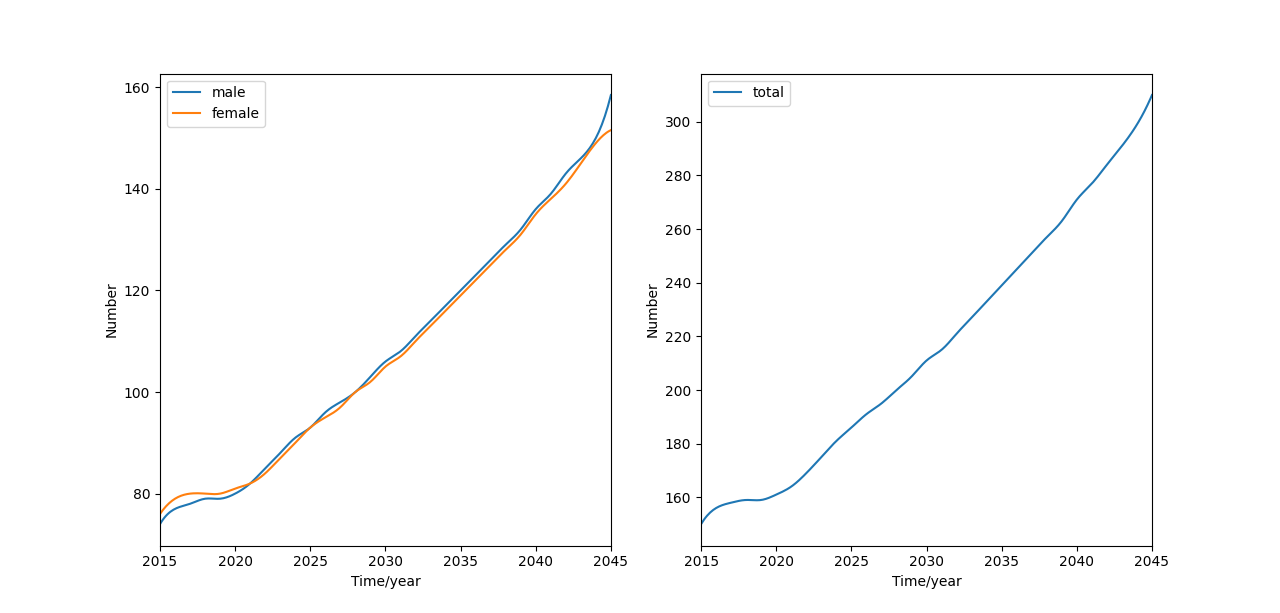
\includegraphics[height=6cm,width=13cm]{figures/prot1.png}%图片名
	\caption{Population changes in protected areas in the next 20 years}%\label{fig:7}%题注
\end{figure}

According to the change curve of the number of finless porpoises in the reserve, it can be seen that the superior living environment of the ex situ reserve provides a good guarantee for the reproduction of the finless porpoise. The average growth rate is increasing year by year, and the population is expected to reach 271 by 2042.

\subsubsection{Sex Ratio Effect}
In order to analyze the effect of sex ratio on the dynamic evolution of finless porpoise population, six groups of male and female ratios were selected, and the female proportions were 0.1, 0.2, 0.4, 0.6, 0.8, and 0.9, respectively, and substituted into the initial state sequence of the hidden Markov model. Then, the change curve of the population of finless porpoise in the next 20 years is obtained :
\begin{figure}[htbp]%插入图片
	\small
	\centering
	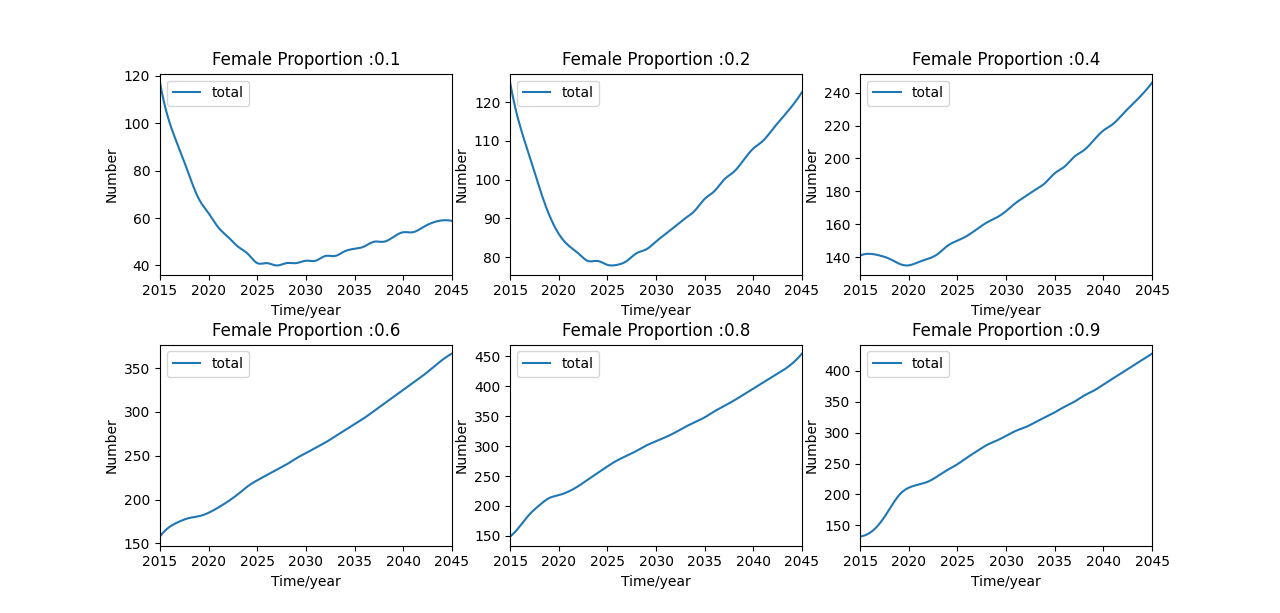
\includegraphics[height=6cm,width=13cm]{figures/sex.png}%图片名
	\caption{The effect of sex ratio on population evolution}%\label{fig:7}%题注
\end{figure}

When the proportion of females is less than 0.5: in the early stage of evolution, due to the small proportion of female individuals, the population reproduction coefficient is low, the number of newborn juveniles in the population is less than the total number of deaths in each age group, and the total number of finless porpoises continues to decline;

With the passage of time, the female ratio of newborn porpoises has basically remained at the level of 1:1, and the lower female-to-male ratio indicates that the mating probability of a single female finless porpoise is higher, which makes the proportion of females in the population continue to rise, and the sex ratio is increasing. Improvement, the population reproduction coefficient increases year by year, so when the reproduction rate begins to catch up with the mortality rate, the population number begins to rise continuously.
And the greater the ratio of males and females, the earlier the inflection point of the curve arrives.

\section{Model 2 : Dynamic evolution model of wild population}
\subsection{Overview of wild population}
Under natural conditions, the survival of dolphins will be threatened by human factors such as shipping, fisheries, water pollution, water conservancy projects and other natural disasters. Meanwhile, due to frequent human activities near Yangtze River, the living space of dolphins will shrink sharply, and the environmental capacity will decrease annually. Therefore, the development of wild dolphin populations needs to consider the impact of those external survival resistance stated above. Compared with ex-situ protection, because of great biodiversity in the wild, the impact of inbreeding depression can be ignored.

According to historical data, the Yangtze River porpoise will soon be extinct unless proper protection. Therefore, it is considered that the unfavorable factors such as shipping, fishery, water quality and hydraulic engineering of the Yangtze River will not change much before the functional extinction of its population, so those factors can be regarded as constants hereinafter.
\begin{figure}[htbp]%插入图片
	\small
	\centering
	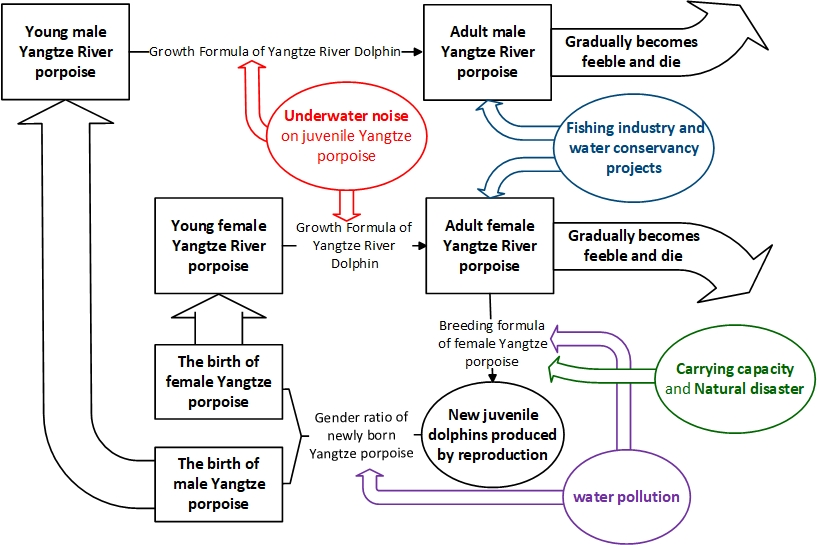
\includegraphics[height=8cm,width=10cm]{figures/2mod.jpg}%图片名
	\caption{Population dynamics model in non-protected areas}%\label{fig:7}%题注
\end{figure}

\subsection{Establishment of dynamic models}
\subsubsection{Population Viability Assessment}
The environmental capacity decreases by $2\%\sim 3\%$ year by year, so the expression of the environmental capacity in the $t$ year is $K(t)={{K}_{0}}-0.025t$. And the population density is:
\begin{equation}
D(t)=N(t)/({{K}_{0}}-0.025t)    
\end{equation}

The snowstorm in 2008 and the drought in Poyang Lake in 2019 caused severe damage to the wild finless porpoise population, indicating that natural disasters are inevitable in non-protected areas. Assume that the probability of natural disasters is $dz$, and the population reproduction rate and the survival rate of newborn dolphins are reduced by 95\%.

The impact of water pollution on finless porpoise is mainly manifested in the decrease of embryo mortality $\alpha $ and the survival rate of male and female juveniles $L{{\eta }_{j}}$ \upcite{5} , resulting in a decrease in the birth rate and sex ratio of the finless porpoise, resulting in a decrease in the wild population. declining.
The survey shows that the mortality rate of water-polluted embryos is roughly 10\%, and the sex ratio of newborn embryos is roughly $1:3.5$
population reproduction rate is:
\begin{equation}
b(t)=0.095\alpha \cdot dz\cdot \frac{{{f}_{1}}(D(t))\cdot {{f}_{2}}({{\eta }_{m}})\cdot {{\eta }_{f}}\Delta {{t}_{breed}}}{(\Delta {{t}_{mature}}+\Delta {{t}_{\text{br}eed}})\Delta {{t}_{birth}}}   
\end{equation}


Assuming that the proportion of hearing loss caused by the underwater noise generated by the shipping industry is ${{H}_{loss}}$, the relevant research results show that the survival probability of the young dolphin after hearing loss is only about 70\% of the original, so The survival rate of each age group under the action of underwater noise is roughly $\text{s}{{\text{1}}_{ij}}(t)=\left[ 1-{3{{H}_{loss} }}/{(1-i)}\; \right]{{s}_{ij}}(0)$, so considering the influence of water pollution, shipping, fishery, natural disasters and other factors, the The expressions are:

\textbf{Survival rate by age:}
\begin{equation}
{{s}_{ij}}(t)=\left( 1-\frac{2.85dz\cdot {{H}_{loss}}\cdot (1-L{{\eta }_{j}})}{1-i} \right){{s}_{ij}}(0)   
\end{equation}


\textbf{The number of dead individuals in the population under natural conditions:}
\begin{equation}
\Delta {{N}_{death}}(t,t+1)=\sum\limits_{i=0}^{16}{N(t){{\omega }_{i-1j}}(t)\cdot {{s}_{ij}}(0)\left( 1-\frac{2.85dz\cdot {{H}_{loss}}\cdot (1-L{{\eta }_{j}})}{1-i} \right)} 
\end{equation}


The number of new male and female individuals in the young dolphins:

\begin{equation}
\begin{aligned}
%\begin{split}
{{\omega }_{i j}}(t+1)= \left \{
\begin{array}{ll}
\Delta Ne{{w}_{f}}=\sum\limits_{i=5}^{16}{0.106dz\cdot {{\omega }_{i1}}(t)\cdot b(t)}\cdot L{{\eta }_{f}},   & female\\
\Delta Ne{{w}_{m}}=\sum\limits_{i=5}^{16}{0.371dz\cdot {{\omega }_{i1}}(t)\cdot b(t)}\cdot L{{\eta }_{m}},  &male
\end{array}
\right.
%\end{split}
\end{aligned}
\end{equation}


Therefore, the population size in t+1 year is:
$N(t+1)=N(t)+\Delta Ne{{w}_{f}}+\Delta Ne{{w}_{m}}-\Delta {{N}_{death}}(t,t+1)$The calculation formulas and iterative relationships of other parameters are consistent with Model 1, and will not be repeated here.

\subsubsection{Functional extinction time prediction}
Based on the definition of the term functional extinct, we give a clear criterion on whether Yangtze River dolphins are in the state of functional extinction.
In Zhang's article, he stated that the minimum viable population for Yangtze River dolphins is 20, so we think that when the population of dolphin is under 20, they become functionally extinct.
\begin{figure}[htbp]%插入图片
	\small
	\centering
	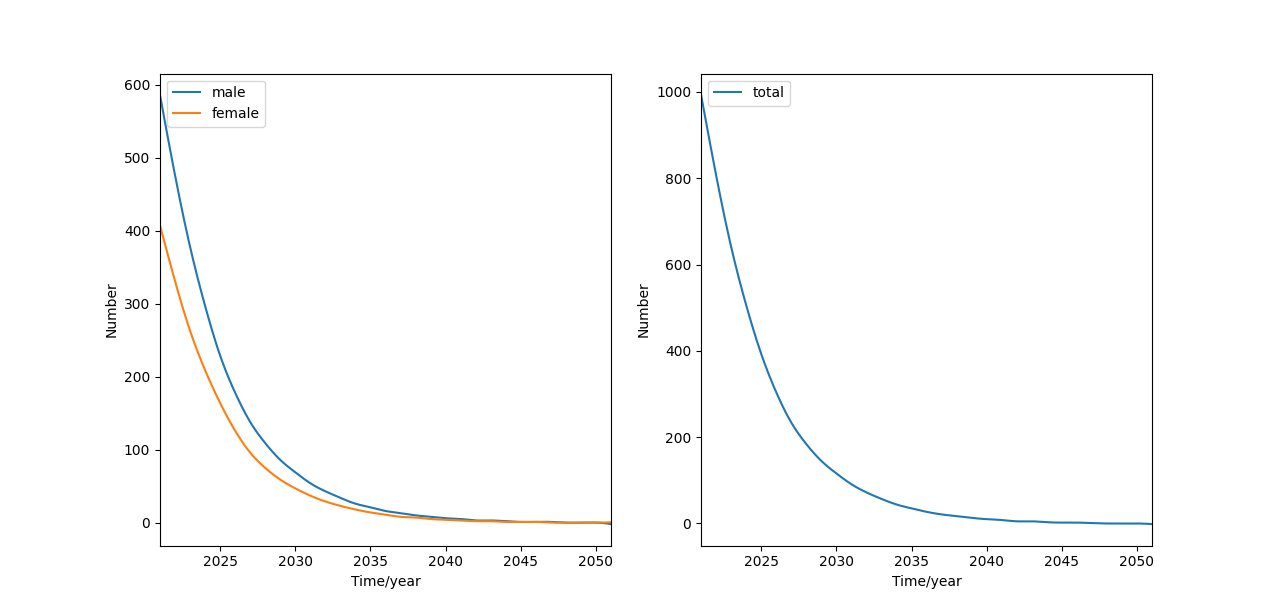
\includegraphics[height=6cm,width=13cm]{figures/notpro.png}%图片名
	\caption{Number of species in non-protected areas}%\label{fig:7}%题注
\end{figure}
Substitute the initial values of the finless porpoise population parameters in Table 5 into the hidden Markov model to obtain the finless porpoise population decay curve without ex situ conservation measures.

According to the prediction results, it can be seen that the population of finless porpoise exhibits an obvious exponential decay trend under the conditions of wild survival. In the early stage of evolution, the population number rapidly decreases with a large decay rate, and the birth rate of the population declines seriously. With a small number of adult and old individuals, the population reproduction rate drops to 0, and functional extinction occurs in 2035.

\section{Sensitivity analysis}
\subsection{Sensitivity analysis of HMM model to shipping industry}
In a non-protected finless porpoise population decline model, underwater noise from the shipping industry reduces the survival rate of juvenile porpoises:
\begin{equation}
\text{s}{{\text{1}}_{i j}}(t)=\left[ 1-{3{{H}_{loss}}}/{(1-i)} \right]{{s}_{i j}}(0)
\end{equation}

In order to test the sensitivity of the non-protected finless porpoise population decline model to the underwater noise generated by the shipping industry, the population evolution curves under the influence of six different noise indices were simulated respectively.

\begin{figure}[htbp]%插入图片
	\small
	\centering
	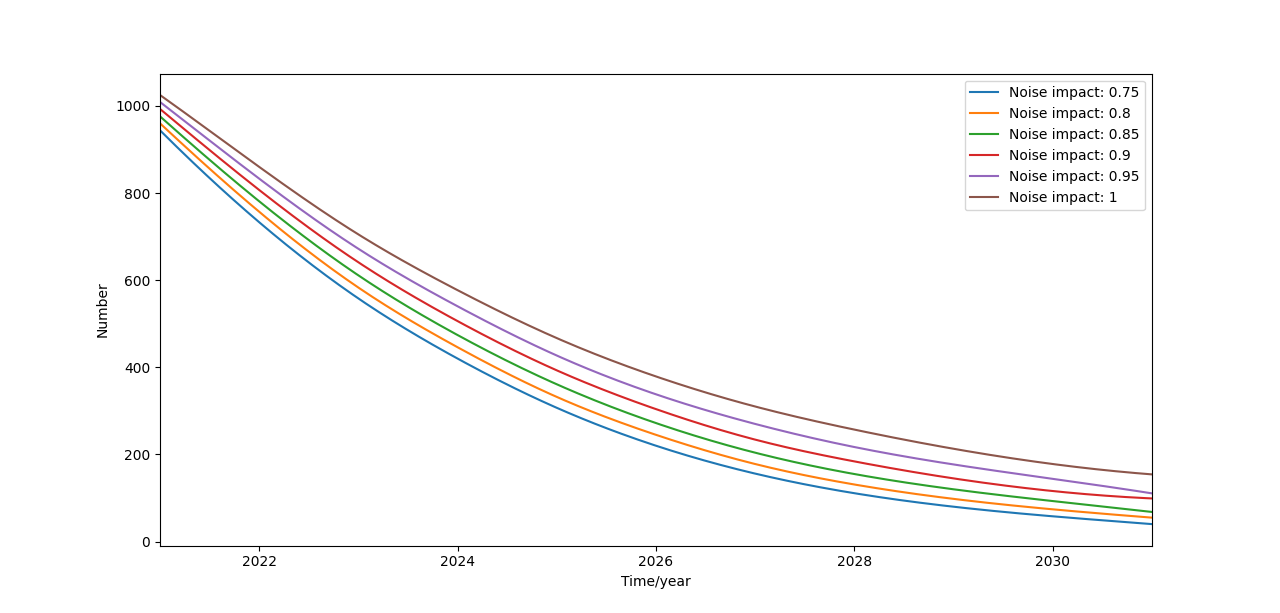
\includegraphics[height=4.5cm,width=13cm]{figures/hear.png}%图片名
	\caption{Underwater noise sensitivity analysis}%\label{fig:7}%题注
\end{figure}

According to the simulation results, it can be seen that with the increase of the underwater noise index, the decay rate of the finless porpoise population is accelerated, indicating that the shipping industry in the model will indeed affect the decline of the finless porpoise population.
\subsection{Sensitivity analysis of HMM model to water pollution}
Combining the reproduction rate\[b(t)=0.095\alpha \cdot dz\cdot b(0)\] and survival rate $s_{{2}_{i j}}\propto (1 -L{{\eta }_{j}})$ expression can be obtained, the aggravation of water pollution will lead to aggravation of population decline.

\begin{figure}[htbp]%插入图片
	\small
	\centering
	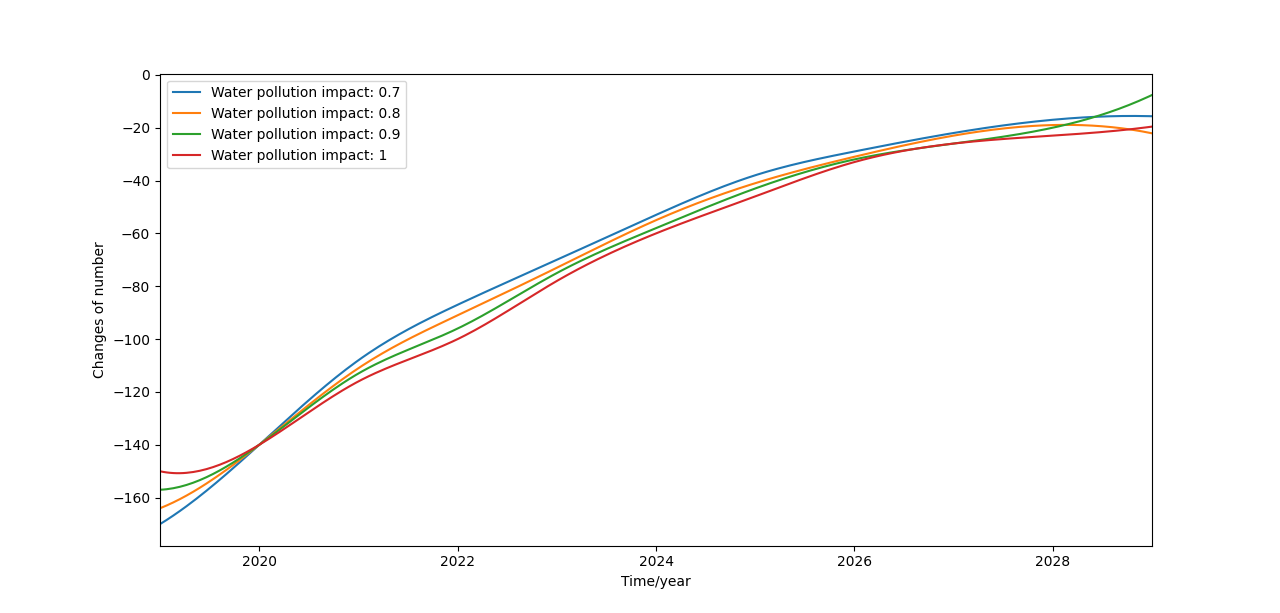
\includegraphics[height=6cm,width=12cm]{figures/watp.png}%图片名
	\caption{Underwater noise sensitivity analysis} %\label{fig:7}%题注
\end{figure}

By simulating the dynamic changes of the finless porpoise population under different water quality, it is concluded that the water quality is also negatively correlated with the decline rate of the population, which verifies the sensitivity of the model to water pollution in the Yangtze River Basin.

\section{Strengths and Weaknesses}
\subsection{Strengths}
\begin{itemize}
    \item Based on the physiological characteristics of the Yangtze River Dolphin, this model comprehensively considered the six internal factors , as well as the five external factors of the Yangtze River shipping industry, fishery, natural disasters, water pollution and environmental capacity. Each proposed factor has its supporting research paper, therefore the establishment of this model is reasonable and has strong practical significance.
    \item Based on the randomness of biological activities, we establish a hidden Markov prediction model.
    All life activities of the porpoise population are described by probability distribution, taking into account the randomness of the fate of small groups. 
    \item By considering about the fact that the breeding mode of finless porpoise is density-restricted, and there is a trend of inbreeding decline, a differential equation system is constructed to comprehensively and reasonably characterize the viability of the protected area population.
\end{itemize}

\subsection{Weaknesses}
\begin{itemize}
    \item The initial state observation sequence of the population is difficult to determine, and a large amount of data needs to be consulted.
    
    \item There are some unknowns in the difference equation system that characterizes the population viability, which needs to be obtained by combining with dynamic programming, and the solution process is complicated.
 \end{itemize}

% 以下为信件/备忘录部分,不需要可自行去掉
% 如有需要可将整个 letter 环境移动到文章开头或中间
% 请在第二个花括号内填写标题,如「信件」(Letter)或「备忘录」(Memorandum)

% 参考文献,此处以 MLA 引用格式为例
\begin{thebibliography}{99}
\bibitem{1} Xianfeng, Zhang, and Wang Kexiong. "Population viability analysis for the Yangtze finless porpoise." Acta Ecologica Sinica 19.4 (1999): 529-533.
\bibitem{2} Yang, Guang, et al. "A study on the life table and dynamics of three finless porpoise populations in the Chinese waters." Oceanographic Literature Review 9.45 (1998): 1640.
\bibitem{3} Lacy, Robert C. "VORTEX: a computer simulation model for population viability analysis." Wildlife research 20.1 (1993): 45-65.
\bibitem{4} Ralls, Katherine, Jonathan D. Ballou, and Alan Templeton. "Estimates of lethal equivalents and the cost of inbreeding in mammals." Conservation biology 2.2 (1988): 185-193.
\bibitem{5} Mei, Zg, Yj Hao, and Js Zheng. "Research progress on population decline mechanism of the endangered Yangtze finless porpoise." Chinese Bulletin of Life Sciences 23.5 (2011): 519-524.

\end{thebibliography}
%\upcite{4}
\begin{letter}{Who can hear the last supplication of the finless porpoise}
\begin{flushleft}  % 左对齐环境,无首行缩进
\textbf{To:} Finless Porpoise Protection Department\\
\textbf{From:} Team XJ210\\
\textbf{Date:} January 17th, 2022\\
\textbf{Subject:} Advice on the protection of finless porpoises
\end{flushleft}
Dear Sir or Madam,

It is our honor to be able to give you several views on the protection of dolphins. Based on the relevant data and the constructed dynamic evolution model of the Yangtze River population, we propose the following suggestions, hoping that you can adopt them.

With the intensification of modern human industrial activities, the ecological environment of the Yangtze River Basin has deteriorated sharply, and the water pollution has become increasingly serious. So the living environment of dolphins has been seriously threatened.

In the past 20 years, the population of Yangtze River dolphins has rapidly declined and entered an extremely endangered state. By constructing the dynamic evolution model of Yangtze River population, we find that, if measures cannot be carried out timely, Yangtze River dolphins are expected to enter an endangered state in 2035, so it is urgent to protect Yangtze River dolphins.


\begin{itemize}
    \item  \textbf{Set up more and more ex-situ refuges}
 \end{itemize}


By comparing the evolution trend of the population of dolphins in the ex situ refuges, it is obvious to conclude that the construction of more ex situ refuges can effectively curb the decline of the population of dolphins in the Yangtze River. What is more, due to the superior natural environment of the relocated protected areas, the population of dolphins is expected to rise back to the safe value.
\begin{figure}[htbp]
\centering
\begin{subfigure}[b]{.4\textwidth}
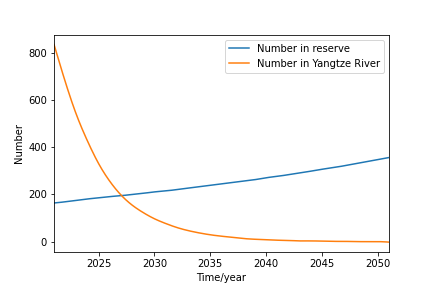
\includegraphics[width=\textwidth]{figures/procom.png}
\caption{Comparison of protected areas}\label{subfig:left}
\end{subfigure}
\begin{subfigure}[b]{.4\textwidth}
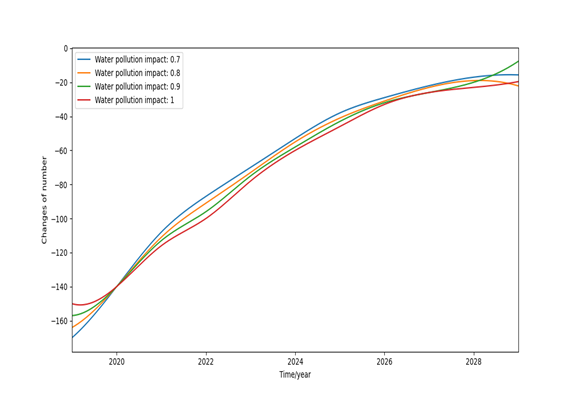
\includegraphics[width=\textwidth]{figures/le2.png}
\caption{The impact of water pollution levels}\label{subfig:right}
\end{subfigure}
%\caption{Two images}\label{fig:subfigures}
\end{figure}

\noindent%取消单段缩进
\textbf{\S  \ Advice to the finless porpoise sanctuary }
 
 Due to the large population density and limited activity range of dolphins in the ex situ refuge, when the population evolution period is long, the influence of inbreeding depression is becoming more and more obvious. The genetic diversity of the population decreases, the frequency of lethal alleles increases, so the survival rate of the offspring decreases year by year. 
 


 \begin{itemize}
    \item  \textbf{Strengthen the management of the original environment of the finless porpoise}
 \end{itemize}
 
 
 There is a stable environment suitable for the growth of finless porpoise after long-term species iteration. Here we can mention the environmental capacity. From a biological point of view, a stable environment has a complete food chain and other factors, and in the long run, it is more suitable for the sustainable development of the finless porpoise population. 
 
 Although the artificial environment is good, the cost is too high (the environmental capacity is not high), and it can only be applied to endangered animals. If you want the finless porpoise to break away from the endangered environment and become a healthy species again, it is not enough to establish a protected area. 
 
 \noindent%取消单段缩进
\textbf{\S  \ Strictly control the scale of fishing in the Yangtze River Basin, and severely suppress the illegal activities of overfishing and illegal fishing }

 
 Overfishing and illegal fishing activities that deplete the fish resources that sustain the baiji and Yangtze finless porpoise have been blamed as one of main reasons for the decline of both species. To protect the remaining fish resources, we suggest that fishing should be forbidden year-round in the entire river; as a minimal initial first step, fishing should be forbidden in all reserves. Furthermore, re-establishing linkage between the Yangtze River and its appended lake clusters could greatly improve the habitat status of fish resources of the river.
 
\noindent%取消单段缩进
\textbf{\S  \ The shipping routes of the Yangtze River basin should be optimized and integrated, and the waterways of the Yangtze River should be used efficiently and greenly }

 
 Aquatic animals use and produce sound for critical life functions, including reproduction and predation. Anthropogenic noise is recognized as a global source of environmental pollution and adequate conservation and management strategies are urgently needed. We cannot abruptly ban the transportation business on Yangtze River because the cost of this proposal is much greater than its price. What we can do is to find the right balance between protecting Yangtze River dolphins and ensuring economic development and achieve sustainable growth. For example, we can optimize transportation efficiency of Yangtze River channel or we can replace ship with other ways of transportation if conditions permit.
 
 
 The above are the suggestions of our team. We hope that people's awareness of environmental protection will continue to increase, and more people will participate in the protection of the Yangtze finless porpoise. One day in the future, our children and grandchildren will be able to see groups of finless porpoises frolicking on the banks of the river.
 
 Sincerely, Team $\#$XJ210
\end{letter}

\newpage
% 以下为附录内容
% 如您的论文中不需要附录,请自行删除

\begin{appendices}

\section{First appendix}

%\inputminted{python}{./code/solve_Q1_1.py}{colorful}

\textbf{\textcolor[rgb]{0.98,0.00,0.00}{Python source of HMM model 1:}}
{\lstinputlisting[language=Python]{./code/solve_Q1_1.py}
}

\section{Second appendix}

\textcolor[rgb]{0.98,0.00,0.00}{\textbf{Python source of HMM model 2:}}
\lstinputlisting[language=Python]{./code/solve_Q2.py}

\end{appendices}

\end{document}  % 结束
